\documentclass{article}
\usepackage{tikz,xcolor,amsmath}
\usepackage[paperwidth=22cm,paperheight=16cm,margin=0.3cm]{geometry}
\usetikzlibrary{arrows.meta}
\pagestyle{empty}
\begin{document}
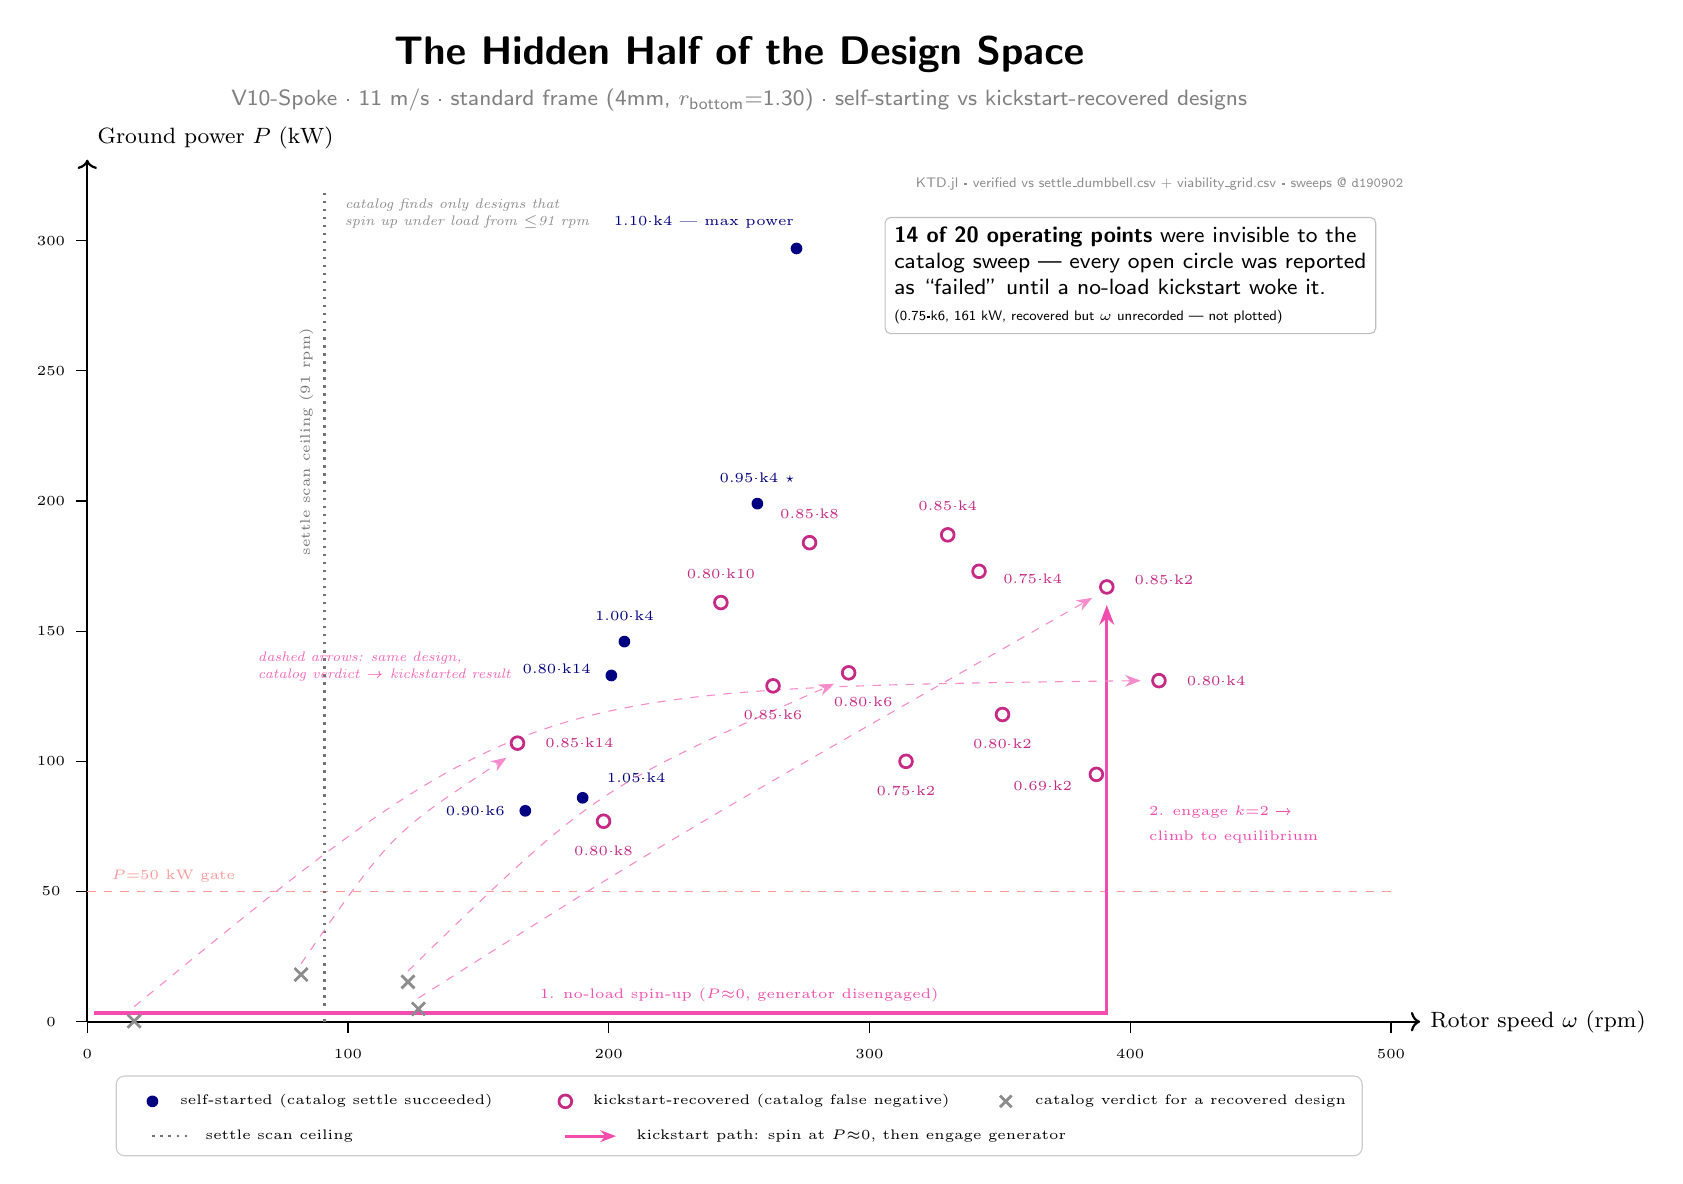
\begin{tikzpicture}[scale=0.92]

% fig4a (2026-07-16): replaces half of the retired fig4. One story, two point classes:
% designs the catalog settle procedure could start vs designs only reachable by
% no-load kickstart. Standard frame only (4mm tether, r_bottom=1.30). No FoS encoding
% (see fig2), no frame variants (see design cards).
% Coordinate maps: x = 2.0 + omega*0.036,  y = 2.0 + P*11.5/320

% ── Title ──
\node[font=\Large\sffamily\bfseries] at (11.0, 15.35) {The Hidden Half of the Design Space};
\node[font=\footnotesize\sffamily, black!50] at (11.0, 14.72) {V10-Spoke · 11 m/s · standard frame (4mm, $r_{\text{bottom}}$=1.30) · self-starting vs kickstart-recovered designs};

% ── Axes ──
\draw[->, thick] (2.0, 2.0) -- (20.4, 2.0) node[right, font=\footnotesize] {Rotor speed $\omega$ (rpm)};
\draw[->, thick] (2.0, 2.0) -- (2.0, 13.9) node[above right, font=\footnotesize] {Ground power $P$ (kW)};
\foreach \w in {0,100,200,300,400,500} {
  \pgfmathsetmacro{\x}{2.0 + \w*0.036}
  \draw (\x, 1.85) -- (\x, 2.0);
  \node[font=\tiny] at (\x, 1.55) {\w};
}
\foreach \p in {0,50,100,150,200,250,300} {
  \pgfmathsetmacro{\y}{2.0 + \p*11.5/320}
  \draw (1.85, \y) -- (2.0, \y);
  \node[font=\tiny] at (1.5, \y) {\p};
}

% ── Gates ──
\pgfmathsetmacro{\pg}{2.0 + 50*11.5/320}
\draw[dashed, red!40] (2.0, \pg) -- (20.0, \pg);
\node[font=\tiny, red!40, anchor=west] at (2.2, {\pg+0.22}) {$P{=}50$ kW gate};

% Settle scan ceiling — the honest replacement for the old pink region:
% the catalog can only discover designs that climb under load from here.
\pgfmathsetmacro{\sc}{2.0 + 91*0.036}
\draw[dotted, black!55, line width=0.9pt] (\sc, 2.0) -- (\sc, 13.5);
\node[font=\tiny, black!55, rotate=90, anchor=west, align=left] at ({\sc-0.25}, 8.3)
  {settle scan ceiling (91 rpm)};
\node[font=\tiny\itshape, black!45, align=left, anchor=west] at ({\sc+0.15}, 13.15)
  {catalog finds only designs that\\spin up under load from $\le$91 rpm};

% ── L-path exemplar: how a kickstart reaches its operating point (0.85·k2) ──
\pgfmathsetmacro{\kx}{2.0 + 391*0.036}
\pgfmathsetmacro{\ky}{2.0 + 167*11.5/320}
\draw[magenta!70, line width=1.1pt, -{Stealth[length=2.5mm]}]
  (2.1, 2.12) -- ({\kx}, 2.12) -- (\kx, {\ky-0.25});
\node[font=\tiny, magenta!70, anchor=south] at (11.0, 2.14) {1. no-load spin-up ($P{\approx}0$, generator disengaged)};
\node[font=\tiny, magenta!70, anchor=west] at ({\kx+0.45}, 4.9) {2. engage $k{=}2$ →};
\node[font=\tiny, magenta!70, anchor=west] at ({\kx+0.45}, 4.55) {climb to equilibrium};

% ══ Catalog false negatives (grey ×) and their kickstart recoveries ══
% Recovery arrows: same design, woken properly.
\def\xmark#1#2{\draw[black!45, line width=1.0pt]
  ({2.0+#1*0.036-0.09}, {2.0+#2*11.5/320-0.09}) -- ({2.0+#1*0.036+0.09}, {2.0+#2*11.5/320+0.09})
  ({2.0+#1*0.036-0.09}, {2.0+#2*11.5/320+0.09}) -- ({2.0+#1*0.036+0.09}, {2.0+#2*11.5/320-0.09});}
\xmark{127}{4.9}   % 0.85k2
\xmark{82}{18.1}   % 0.85k14
\xmark{123}{15.3}  % 0.80k6
\xmark{18}{0.2}    % 0.80k4
\node[font=\tiny, black!45, anchor=north] at ({2.0+82*0.036}, 2.5) {};

% Recovery arrows (dashed, thin, curved)
\draw[magenta!45, dashed, -{Stealth[length=2mm]}] ({2.0+127*0.036}, {2.0+4.9*11.5/320+0.15})
  .. controls (10.0, 4.5) .. ({2.0+391*0.036-0.2}, {2.0+167*11.5/320-0.15});
\draw[magenta!45, dashed, -{Stealth[length=2mm]}] ({2.0+82*0.036}, {2.0+18.1*11.5/320+0.15})
  .. controls (6.2, 4.6) .. ({2.0+165*0.036-0.15}, {2.0+107*11.5/320-0.2});
\draw[magenta!45, dashed, -{Stealth[length=2mm]}] ({2.0+123*0.036}, {2.0+15.3*11.5/320+0.15})
  .. controls (9.0, 5.2) .. ({2.0+292*0.036-0.2}, {2.0+134*11.5/320-0.15});
\draw[magenta!45, dashed, -{Stealth[length=2mm]}] ({2.0+18*0.036}, {2.0+0.2*11.5/320+0.2})
  .. controls (8.0, 6.6) .. ({2.0+411*0.036-0.25}, {2.0+131*11.5/320});
\node[font=\tiny\itshape, magenta!60, align=left] at (6.1, 6.9)
  {dashed arrows: same design,\\catalog verdict → kickstarted result};

% ══ Point classes ══
% \self{omega}{P} — catalog self-started (filled dark blue)
\def\selfpt#1#2{\fill[blue!50!black] ({2.0+#1*0.036}, {2.0+#2*11.5/320}) circle (2.3pt);}
% \kick{omega}{P} — kickstart-recovered (open magenta)
\def\kickpt#1#2{\draw[magenta!80!black, line width=1.0pt, fill=white]
  ({2.0+#1*0.036}, {2.0+#2*11.5/320}) circle (2.5pt);}

% Self-started (6)
\selfpt{168}{81}   \node[font=\tiny, blue!50!black, anchor=east]  at ({2.0+168*0.036-0.15}, {2.0+81*11.5/320})  {0.90·k6};
\selfpt{201}{133}  \node[font=\tiny, blue!50!black, anchor=east]  at ({2.0+201*0.036-0.15}, {2.0+133*11.5/320+0.1}) {0.80·k14};
\selfpt{206}{146}  \node[font=\tiny, blue!50!black, anchor=south] at ({2.0+206*0.036}, {2.0+146*11.5/320+0.15}) {1.00·k4};
\selfpt{190}{86}   \node[font=\tiny, blue!50!black, anchor=west]  at ({2.0+190*0.036+0.2}, {2.0+86*11.5/320+0.28}) {1.05·k4};
\selfpt{257}{199}  \node[font=\tiny, blue!50!black, anchor=south] at ({2.0+257*0.036}, {2.0+199*11.5/320+0.15}) {0.95·k4 $\star$};
\selfpt{272}{297}  \node[font=\tiny, blue!50!black, anchor=south east] at ({2.0+272*0.036+0.1}, {2.0+297*11.5/320+0.15}) {1.10·k4 — max power};

% Kickstart-recovered (13)
\kickpt{165}{107}  \node[font=\tiny, magenta!80!black, anchor=west] at ({2.0+165*0.036+0.25}, {2.0+107*11.5/320}) {0.85·k14};
\kickpt{198}{77}   \node[font=\tiny, magenta!80!black, anchor=north] at ({2.0+198*0.036}, {2.0+77*11.5/320-0.2})  {0.80·k8};
\kickpt{243}{161}  \node[font=\tiny, magenta!80!black, anchor=south] at ({2.0+243*0.036}, {2.0+161*11.5/320+0.2}) {0.80·k10};
\kickpt{263}{129}  \node[font=\tiny, magenta!80!black, anchor=north] at ({2.0+263*0.036}, {2.0+129*11.5/320-0.2}) {0.85·k6};
\kickpt{277}{184}  \node[font=\tiny, magenta!80!black, anchor=south] at ({2.0+277*0.036}, {2.0+184*11.5/320+0.2}) {0.85·k8};
\kickpt{292}{134}  \node[font=\tiny, magenta!80!black, anchor=north] at ({2.0+292*0.036+0.2}, {2.0+134*11.5/320-0.2}) {0.80·k6};
\kickpt{314}{100}  \node[font=\tiny, magenta!80!black, anchor=north] at ({2.0+314*0.036}, {2.0+100*11.5/320-0.2}) {0.75·k2};
\kickpt{330}{187}  \node[font=\tiny, magenta!80!black, anchor=south] at ({2.0+330*0.036}, {2.0+187*11.5/320+0.2}) {0.85·k4};
\kickpt{342}{173}  \node[font=\tiny, magenta!80!black, anchor=west]  at ({2.0+342*0.036+0.2}, {2.0+173*11.5/320-0.1}) {0.75·k4};
\kickpt{351}{118}  \node[font=\tiny, magenta!80!black, anchor=north] at ({2.0+351*0.036}, {2.0+118*11.5/320-0.2}) {0.80·k2};
\kickpt{387}{95}   \node[font=\tiny, magenta!80!black, anchor=east] at ({2.0+387*0.036-0.2}, {2.0+95*11.5/320-0.15})  {0.69·k2};
\kickpt{391}{167}  \node[font=\tiny, magenta!80!black, anchor=west]  at ({2.0+391*0.036+0.25}, {2.0+167*11.5/320+0.1}) {0.85·k2};
\kickpt{411}{131}  \node[font=\tiny, magenta!80!black, anchor=west]  at ({2.0+411*0.036+0.25}, {2.0+131*11.5/320})  {0.80·k4};

% ── Key takeaway ──
\node[font=\footnotesize\sffamily, align=left, draw=black!25, rounded corners=2pt, fill=white] at (16.4, 12.3)
  {\textbf{14 of 20 operating points} were invisible to the\\
   catalog sweep — every open circle was reported\\
   as ``failed'' until a no-load kickstart woke it.\\
   {\tiny (0.75·k6, 161 kW, recovered but $\omega$ unrecorded — not plotted)}};

% ── Legend ──
\draw[rounded corners=3pt, fill=white, draw=gray!40] (2.4, 0.15) rectangle (19.6, 1.25);
\fill[blue!50!black] (2.9, 0.9) circle (2.3pt);
\node[font=\tiny, anchor=west] at (3.15, 0.9) {self-started (catalog settle succeeded)};
\draw[magenta!80!black, line width=1.0pt, fill=white] (8.6, 0.9) circle (2.5pt);
\node[font=\tiny, anchor=west] at (8.85, 0.9) {kickstart-recovered (catalog false negative)};
\draw[black!45, line width=1.0pt] (14.6,0.82) -- (14.76,0.98) (14.6,0.98) -- (14.76,0.82);
\node[font=\tiny, anchor=west] at (14.95, 0.9) {catalog verdict for a recovered design};
\draw[dotted, black!55, line width=0.9pt] (2.9, 0.42) -- (3.4, 0.42);
\node[font=\tiny, anchor=west] at (3.5, 0.42) {settle scan ceiling};
\draw[magenta!70, line width=1.1pt, -{Stealth[length=2mm]}] (8.6, 0.42) -- (9.3, 0.42);
\node[font=\tiny, anchor=west] at (9.45, 0.42) {kickstart path: spin at $P{\approx}0$, then engage generator};

% ── Provenance ──
\node[font=\tiny\sffamily, black!45, anchor=south east] at (20.3, 13.35)
  {KTD.jl · verified vs settle\_dumbbell.csv + viability\_grid.csv · sweeps @ \texttt{d190902}};

\end{tikzpicture}
\end{document}
